% Intended LaTeX compiler: xelatex
\documentclass[a4paper, 12pt]{article}
\usepackage{graphicx}
\usepackage{longtable}
\usepackage{wrapfig}
\usepackage{rotating}
\usepackage[normalem]{ulem}
\usepackage{amsmath}
\usepackage{amssymb}
\usepackage{capt-of}
\usepackage{hyperref}
\usepackage[danish]{babel}
\usepackage{mathtools}
\usepackage[margin=2.0cm]{geometry}
\hypersetup{colorlinks, linkcolor=black, urlcolor=blue}
\setlength{\parindent}{0em}
\parskip 1.5ex
\author{Jacob Debel}
\date{Fysik C \& B}
\title{Lys og bølger\\\medskip
\large Konstruktion - Avancerede opgaver}
\hypersetup{
 pdfauthor={Jacob Debel},
 pdftitle={Lys og bølger},
 pdfkeywords={},
 pdfsubject={},
 pdfcreator={Emacs 29.4 (Org mode 9.6.15)}, 
 pdflang={Danish}}
\begin{document}

\maketitle



\section*{Opgave 1}
\label{sec:org3a39aba}

Lyset fra en natriumlampe indeholder en kraftig gul dobbeltspektrallinje, hvor de to linjer har en
bølgelængde på hhv. 589.0 nm og 589.6 nm.

Lyset sendes nu igennem et gitter med 600 streger pr. mm. og afbøjningsstrålerne rammer en
bagvedliggende væg. Den oprindelige lysstråle sendes vinkelret ind på både gitter og bagvæg.

\begin{itemize}
\item I hvilke vinkler ses 1.ordens afbøjningerne? (Altså for begge bølgelængder.)
\end{itemize}

For at kunne skelne de to dobbeltlinjer fra hinanden skal de være separeret med 4 mm.

\begin{itemize}
\item Hvor stor en afstand skal der være mellem gitter og bagvæg, for at de to 1.ordens afbøjningsstråler netop er separeret med 4 mm.?
\end{itemize}

\section*{Opgave 2:}
\label{sec:orgc329388}

Røntgenstråling er en del af det elektromagnetiske spektrum og repræsenterer et frekvensinterval fra \(3 \cdot 10^{16}\) Hz til \(3\cdot 10^{19}\) Hz.

\begin{itemize}
\item Hvilket bølgelængdeinterval svarer ovenstående frekvensinterval til?
\end{itemize}

Betragt nu røngtenstråling med en frekvens på \(5.0\cdot 10^{18}\) Hz . Der ønskes et gitter, som kan
udføre en 1.ordens afbøjning på 30 grader.

\begin{itemize}
\item Bestem den nødvendige gitterkonstant for ovenstående gitter.

\item Redegør for, om det er muligt at producere det ønskede gitter, når den interatomare afstand i krystaller typisk er 1-2 Å ( Å = Ångstrøm = 0.1 nm = \(10^{-10} m\)).
\end{itemize}
\newpage

\section*{Opgave 3}
\label{sec:orga83560a}

Med det formål at bestemme vands brydningsindeks fastgøres et optisk gitter på den ene endeflade af et kasseformet glaskar. På den anden endeflade anbringes et stykke papir som skærm. Afstanden mellem gitter og skærm er 40.2 cm.

I et tomt kar sendes laserlys med bølgelængden 632.8 nm vinkelret gennem gitteret. Afstanden mellem de to førsteordenspletter på skærmen er da 21.0 cm.

\begin{itemize}
\item Bestem gitterkonstanten.
\end{itemize}

Der fyldes vand i karret, og afstanden mellem de to førsteordenspletter er nu 15.8 cm.

\begin{itemize}
\item Beregn laserlysets bølgelængde i vand.

\item Bestem på grundlag af denne måling vandets brydningsindeks.
\end{itemize}

\section*{Opgave 4}
\label{sec:org624790b}

En lysstråle sendes vandret ind mod en plan glasklods, som danner en vinkel på \(37^\circ\) med lodret. Glasset har et brydningsindeks på 1.66.

\begin{center}

\includegraphics[width=.9\linewidth]{./img/glasklods.png}
\end{center}

\begin{itemize}
\item Hvilken vinkel danner lysstrålen med vandret inde i glasset?

\item Hvilken vinkel danner strålen med vandret, når den er passeret ud igennem glasset igen?
\end{itemize}

\newpage
\section*{Opgave 5}
\label{sec:orgad6e349}

En person står ved en dam og betragter en fisk (punktet F) på bunden af dammen. Personens øje befinder sig i punktet A, som er 1.7 m over vandoverfladen.

\begin{center}
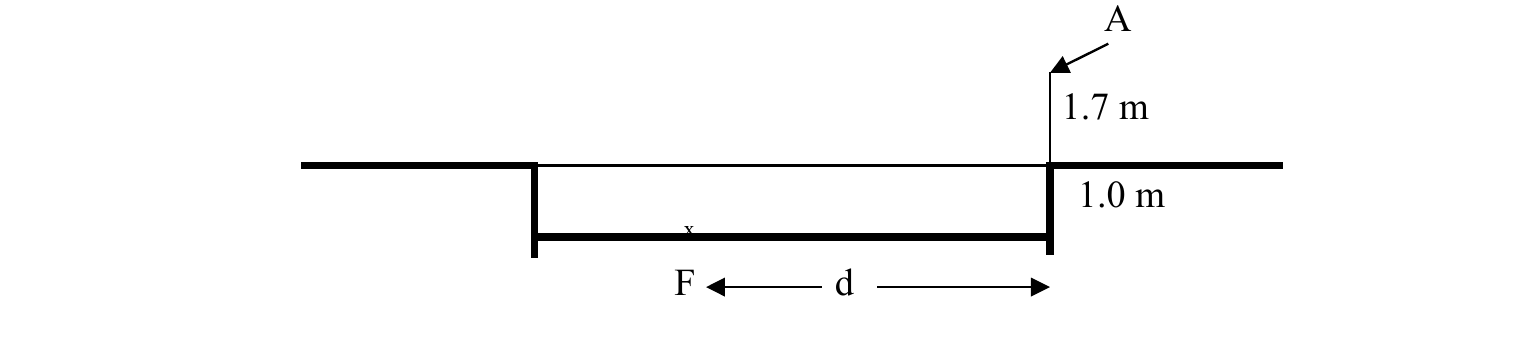
\includegraphics[width=.9\linewidth]{./img/dam.png}
\end{center}

\begin{itemize}
\item Skitsér strålegangen fra A til F.

\item Bestem den vandrette afstand, \(d\), mellem fisken og personen, når personen ser fisken under en vinkel på \(30^\circ\) med vandret, og dammen er 1.0 m dyb.
\end{itemize}
\end{document}
